\subsection{Функция Грина уравнения Лапласа первой краевой задачи в круге, на полуплоскости в полупространстве. Метод отражений.}
%autor: Сеня

\paragraph{Метод отражений (метод электростатических изображений).}\footnote{Т.-С. стр. 343}

Для построения функции источника в виде
\begin{equation*}
	G(M, M_0) = \frac{1}{4 \pi R_{M M_0}} + v
\end{equation*}
индуцированное поле $v$ представляется как поле зарядов, расположенных вне поверхности $\Sigma$ и выбираемых таким образом, чтобы выполнялось условие
\begin{equation*}
	v|_{\Sigma} = -\frac{1}{4 \pi R}.
\end{equation*}

Приведем примеры построения функции источника методом отражений.

Пусть дана сфера радиуса $R$ с центром в точке $O$.

Поместим в точку $M_0$ единичный заряд и отложим на радиусе, проходящем через точку $M_0$, такой отрезок $OM_1$, что
\begin{equation} \label{section}
	\rho_0 \rho_1 = R^2,
\end{equation}
где $\rho_0 = \abs{OM_0}$ и $\rho_1 = \abs{OM_1}$. 

\begin{figure}[H]
	\centering
	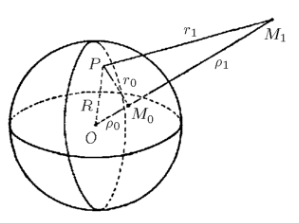
\includegraphics[width=0.4\linewidth]{img/sphere_green}
	\caption{}
\end{figure}

Точки $M_0$ и $M_1$ называются сопряженными друг другу. 

Докажем, что для всех точек $P$ на сфере, расстояния до $M_0$ и $M_1$ пропорциональны. Рассмотрим $\triangle OPM_0$ и $\triangle OMP_1$. Они подобны по общему углу и двум пропорциональным сторонам
\begin{equation*}
	\frac{\rho_0}{R} = \frac{R}{\rho_1}, \text{ или } \frac{\abs{OM_0}}{R} = \frac{R}{\abs{OM_1}}.
\end{equation*}
Из подобия следует
\begin{equation} \label{prop}
	\frac{r_0}{r_1} = \frac{\rho_0}{R} = \frac{R}{\rho_1},
\end{equation}
где $r_0 = \abs{\overrightarrow{M_0P}}$, $r_1 = \abs{\overrightarrow{M_1 P}}$. Из пропорции \eqref{prop} получаем  
\begin{equation*}
	r_0 = \frac{\rho_0}{R} r_1
\end{equation*}
для всех точек сферы. Поэтому гармоническая функция $v = -R/\rho_0 \cdot 1/r_1$ на сфере принимает то же значение, что и функция $-1/r_0$. она представляет, очевидно потенциал заряда величины $-R/\rho_0$, помещенного в точку $M_1$.

Таким образом 
\begin{equation} \label{final_green}
	G(P, M_0) = \frac{1}{4 \pi} \Bigg(\frac{1}{r_0} - \frac{R}{\rho_0} \frac{1}{r_1}\Bigg)
\end{equation}

\paragraph{Функция источника для круга.}\footnote{Т.-С. стр. 346}

Функция источника для круга может быть получена таким же способом, как и функция источника для сферы. В этом случа ее следует искать в виде
\begin{equation}
	G = \frac{1}{2 \pi} \ln{\frac{1}{r}} + v.
\end{equation}

Повторяя рассуждения от \eqref{section} до \eqref{final_green}, мы найдем функцию $G$ в виде 
\begin{equation}
	G = \frac{1}{2 \pi} \Bigg[\ln{\frac{1}{r_0}} - \ln{\frac{R}{\rho_0} \frac{1}{r_1}}\Bigg],
\end{equation}
где $\rho_0 = \abs{OM_0}$, $r_0 = \abs{M_0 P}$, $r_1 = \abs{M_1 P}$, $R = \abs{OP}$ --- радиус круга (см. рис. \ref{circle_green}).
\begin{figure}[H]
	\centering
	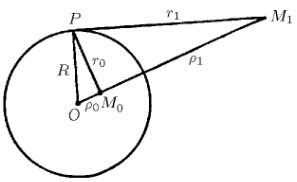
\includegraphics[width=0.4\linewidth]{img/circle_green}
	\caption{}
	\label{circle_green}
\end{figure}
Нетрудно убедиться в том, что определенная таким образом гармоническая функция обращается в нуль на границе: $G|_{C} = 0$.

\paragraph{Функция источника для полупространства.}\footnote{Т.-С. стр. 347}

Найдем функцию источника для полупространства $z > 0$. Поместим в точку $M_0(x_0, y_0, x_0)$ единичный заряд, который создает в неограниченном пространстве поле, потенциал которого определяется функцией 
\begin{equation*}
	\frac{1}{4 \pi} \frac{1}{R_{M_0 M}}, \text{ где } R_{M_0 M} = \sqrt{(x - x_0)^2 + (y - y_0)^2 + (z - z_0)^2}.
\end{equation*}
Нетрудно видеть, что "индуцированное поле" $v$ является полем отрицательного единичного заряда, помещенного в точку $M_1(x_0, y_0, -z_0)$, являющуюся зеркальным изображением точки $M_0$ в плоскости $z = 0$ (рис. \ref{halfdim_green}). 
Функция $G$, равная
\begin{equation*}
	G(M, M_0) = \frac{1}{4 \pi R_0} - \frac{1}{4 \pi R_1},
\end{equation*}
где
\begin{align*}
	R_0 = \abs{\overrightarrow{M_0 M}} = \sqrt{(x - x_0)^2 + (y - y_0)^2 + (z - z_0)^2}, \\
	R_1 = \abs{\overrightarrow{M_1 M}} = \sqrt{(x - x_0)^2 + (y - y_0)^2 + (z - z_0)^2}, \\
\end{align*}
обращается в нуль при $z = 0$ и имеет нужную особенность в точке $M_0$.

\begin{figure}[H]
	\centering
	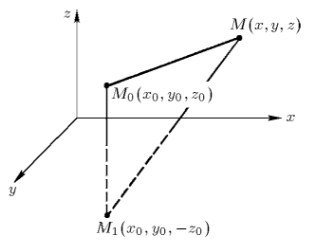
\includegraphics[width=0.4\linewidth]{img/halfdim_green}
	\caption{}
	\label{halfdim_green}
\end{figure}